\section{Experiment Results}
We have conducted experiments on three datasets, where each dataset is obtained by monitoring 24-hour activities of two adults in a house via RFID. 
All these activities occur in twelve rooms; the basement, bathroom, bedroom, dining room, hallway, kitchen, living room, mudroom, nursery, outside-front, outside-back, and upstairs.  
%\begin{table}[h]
%\centering
%\caption{Datasets summary.} 
%\label{tab_dataset}}
%\begin{tabular} {|c|c|c|c|}
%\hline
%Dataset & Number of entries & Period(day) & Start date\\
%\hline
%study10  & 6596 & 12 & 02/10/2014\\
%\hline
%study11  & 1696 & 10 & 01/29/2014\\
%\hline
%study14 & 3453 & 13 & 12/09/2013\\
%\hline
%\end{tabular}
%\end{table}
The dataset comprises events in the form of timestamped room occupancy data points. For instance, an event can correspond to person 1 being in the kitchen at 7:00 am. The summary of these three datasets is shown in Table~\ref{tab_dataset}.
%Study10 spans 12 days from 02/10/2014 to 02/21/2014 and Study11 spans 10 days from 01/29/2014 to 02/07/2014, and Study14 spans 13 days from 12/09/2013 to 12/21/2013.
We define \textit{unoccupancy} of a person as one of these conditions: the person leaves the {\em outside-front} or {\em outside-back} for more than 30 minutes; the person stays in the living room or dining room for more than 9 hours without any other activities; or the gap between any two events is more than 30 minutes. 
Since our research goal is to automate the turning on and off of the HVAC system at least 30 minutes before occupancy, the first and third constraints are in place. We are only interested in events where the {\em unocupancy} period is for an extended duration ($>$ 30 minutes). The second constraint comes from our observation that if a person stays in one room for more than 9 hours without moving to other rooms, 
this usually means that the person has gone out but left the RFID equipment at home. 
Furthermore, we delete events with a duration less than 
2 minutes since these correspond to the individual walking back and forth across rooms and generally do not contribute to meaningful episodes. We conduct four types of experiments to compare four approaches; 
kNN, mixture EGH, PDF, and support vector regression (SVR). 
For each dataset, we use $2/3$ of the data for training and the remaining $1/3$ of the data as a test. 
Following the approach in~\cite{scott2011preheat},
we organize one day's data into 96 15-minute chunks. 
For the test data, we assume that we only know some of the 15-minute chunks. Our target is to predict the occupancy in the rest of the day, or 30 minutes ahead. 

\subsection{Occupancy Prediction of Individuals}
%We apply three approaches, kNN, PDF based and mixture EGH time prediction model. 
%Similar to \cite{scott2011preheat},
%we organize one day's date into 96 15-minutes intervals with mixture EGH model. 
%Then we split the test date into three phases: 
%(1) before getting up, (2) after getting up and before going out, 
%(3) after going out and before coming back. 
%Thus our problem becomes to predict when the person going out 
%and when the person comes back. 
%Corresponding to these four phases, we adopt three different approaches. 
%For stage (1), the probability density function of going out and combing back event is calculated. 
%For stage (2), a duration-constraint episode mining and episode generative HMM is applied. 
%For stage (3), the probability density function of backing time based on 
%the time-constrains going out time is computed. 

%The results are shown in Figure~\ref{fig_study10} and Table~\ref{tab_individualResults}
%Figure~\ref{fig_study11}, and Figure~\ref{fig_study14}. 
%Each of these figures 

\begin{table*}[t]
%\vspace{0.2cm}
\hfill
%\begin{minipage}[t]{1.0\linewidth}%

\caption{Precision Recall F-measure Comparison of Individual and Whole House Occupancy Prediction in Study 14.}
\label{tab_individualResults}
%\tbl{Precision Recall F-measure Comparison of Individual and Whole House Occupancy Prediction in Study 14.\label{tab_individualResults}}{
%\begin{center}
%\makebox[\textwidth]{
\centering
\small
\setlength\tabcolsep{2pt}
\begin{tabular} {|l|l|l|l|l|l|l|l|l|l|l|l|l|l|l|l|}
\hline
\multirow{2}{*}{Dataset}&\multirow{2}{*}{Date}&\multirow{2}{*}{Person} & \multicolumn{3}{|c|}{EGH}&\multicolumn{3}{|c|}{kNN} &\multicolumn{3}{|c|}{SVM}   \\
\cline{4-12}
&&& precision & recall &fmeasure &precision & recall & fmeasure &precision & recall & fmeasure \\
\hline
\multirow{3}{*}{study10}  & 02/17/2014 & person2& \textbf{1.00} & \textbf{1.00}&\textbf{1.00} & 0.99 & 0.98 & 0.98 &0.71 &0.76 & 0.71\\
\cline{2-12}
& 02/19/2014 & person1& 0.98 & 0.99 &0.98&  \textbf{0.99} &  \textbf{0.99} &  \textbf{0.99} & 0.71 & 0.76 & 0.70 \\
\cline{2-12}
& 02/20/2014 & person2&  \textbf{0.93} &  \textbf{0.92} &  \textbf{0.92} & 0.92 & 0.91 & 0.90 & 0.72 & 0.77 & 0.72\\
\cline{2-12}
& 02/20/2014 & person1&  \textbf{0.95}& \textbf{0.94} & \textbf{0.94} & 0.94	& 0.93 & 0.93 & 0.71 & 0.77 & 0.72 \\
\cline{2-12}
& 02/20/2014 & \textbf{wholehouse}&  \textbf{0.92}& \textbf{0.92} & \textbf{0.91} & 0.91	& 0.89 & 0.91 & 0.79 & 0.74 & 0.74 \\
\hline
\hline
\multirow{3}{*}{study11}  & 02/04/2014 & person2& 0.93 & 0.93 & 0.92  & \textbf{0.95} & \textbf{0.95} & \textbf{0.95} & 0.71 & 0.77 &0.72\\
\cline{2-12}
& 02/04/2014 & person1& 0.93 & 0.93 & 0.92  & \textbf{0.95} & \textbf{0.95} & \textbf{0.95} & 0.70 & 0.77 & 0.71  \\
\cline{2-12}
& 02/05/2014 & person2&  \textbf{0.85} &  \textbf{0.92} &  \textbf{0.86} & 0.87 & 0.87 & 0.84 & 0.71 & 0.76 & 0.71 \\
\cline{2-12}
& 02/05/2014 & person1&  \textbf{0.84} &  \textbf{0.90} &  \textbf{0.84} & 0.79 & 0.90 & 0.80  & 0.70 & 0.77 & 0.71   \\
\cline{2-12}
& 02/04/2014 & \textbf{wholehouse}&  \textbf{0.918}& \textbf{0.924} & \textbf{0.913} & 0.916	& 0.921 & 0.911 & 0.77 & 0.69 & 0.71  \\
\cline{2-12}
& 02/05/2014 & \textbf{wholehouse}&  \textbf{0.90}& \textbf{0.84} & \textbf{0.84} & 0.88	& 0.81 & 0.81 & 0.74 & 0.70 & 0.70\\
\hline
\end{tabular}
%}
%\end{center}
%\end{minipage}%
%\hfill%
\end{table*}
The individual occupancy prediction results on datasets Study10 and Study11 are summarized in Table~\ref{tab_individualResults}. 
In Study10,  the mixture EGH performs better than kNN for the occupancy prediction for person2 on 02/17/2014. 
Furthermore, mixture EGH outperforms kNN for both persons on 02/20/2014. 
However, for person1 on 02/19/2014, kNN works a little bit better. 
When checking the original data on this test date, 
we find that the activities on this date are very similar to the historical activities in the training data.
%\textbf{When checking the original data, we find that the date on that day is similar to the historical data. - need to rephrase}
This observation leads us to the conclusion that when the test data is very highly similar to the historical data, 
the kNN approach sometimes performs a little better.  
In Study11, mixture EGH gets higher precision, recall and f-measure scores on 02/05/2014, but the opposite is true on 02/04/2014. 
We analyzed the original data to find the reason for the kNN's better performance, and found the date is an anomaly from the normal pattern, since both individuals went to sleep late that day (after 12:00am).
Before sleep, person1 even stayed in the kitchen for around two hours. 
The frequent episode $KZ$, which represents 'kitchen-unoccupied', 
usually occurs in the morning instead of around midnight. 
However, the mixture EGH model still assumes that the $KZ$ pattern 
happens during the morning; 
therefore the prediction results are not accurate. 
%\textbf{On the contrary, 
%kNN doesn't consider the 
%actual place inside the room. - need to rephrase}
Since kNN ignores this fine granular activity pattern at a house and only considers the occupancy status in the past most similar five days, its performance is better. 
Generally speaking, the mixture EGH helps predict when a person 
leaves home and the period of sleeping and its 
performance is competitive to the kNN approach. 
For all these experiments, the SVR approach performs the worst because 
of the limitations of this approach. 
SVR uses the latest several data points about the occupancy state as the 
training vector for the prediction of the next occupancy state. 
Here we set eight past data points as the predictor. 
Other features such as the time of day and day of week cannot be utilized fully. 

We also conduct experiments for individuals' {\em rest-of-day} occupancy prediction at different times. 
\begin{figure}[h]
\centering
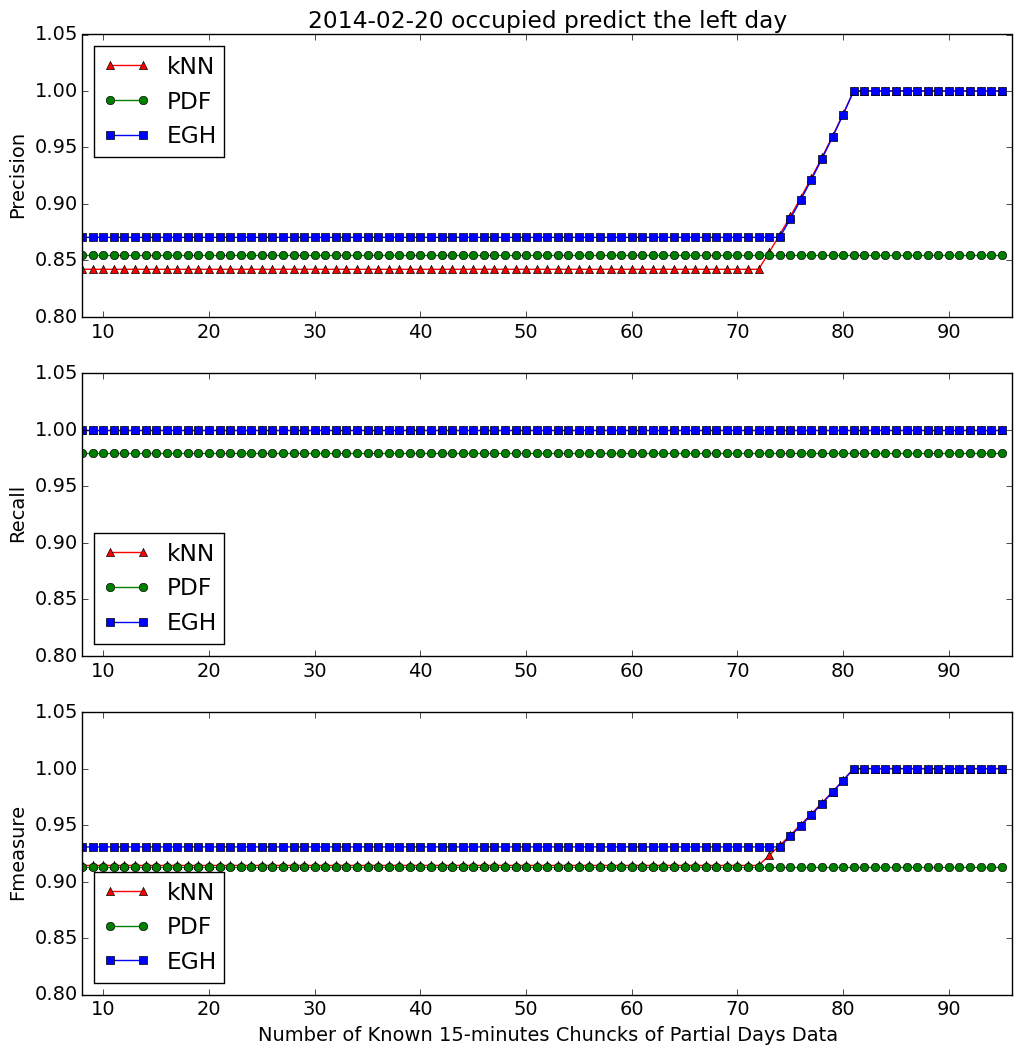
\includegraphics[width=0.5\textwidth]{adlfigs/study10person12014-02-20occupied.png}
\caption{Occupancy prediction precision, recall and f-measure comparison of three approaches 
of person1 on 02/20/2014 on Study10.}
\label{fig_study10}
\end{figure}
Figure~\ref{fig_study10} illustrates a person's occupancy prediction result in Study10.
There are three sub-figures. 
Each sub-figure describes the 
precision, recall, and f-measure 
of $person1$ on 02/20/2014. 
The blue line represents the mixture EGH model,
the green line represents the PDF model,
and the red line denotes the kNN model. 
The x-axis is the number of known 15-minute chunks of the test day. 
For instance, at $x=20$, 
we already know $20*15$ minutes' data 
and need to predict whether the home is occupied during the remaining $76$ chunks. 
The y-axis denotes the precision, recall and f-measure values 
in the three sub-figures from the top down. 
The first sub-figure shows that  
the mixEGH has the highest precision, recall and f-measure on test day 02/20/2014 
for occupancy prediction. The other two baseline approaches are comparable, except that kNN performs better than PDF 
when the person comes back home after slot 72. 
Looking into the original data, we find that person1 actually comes home later than usual 
in the training dataset. 
%In such case, mixture EGH performs best.  
%Figure \ref{fig_study10} (c) and (d) gives the occupancy and un-occupancy results 
%of person2 on 02/17/2014. 
%In such case, EGH mixture model performs best from the perspective of precision, recall and f-measure. 

\iffalse
Figure~\ref{fig_study14} (a) and (b) describe the case of person1 on 12/18/2013. 
Similar to Figure \ref{fig_study11} (a) and (b), 
mixture EGH model doesn't perform well before the person1 gets up 
and the reason keeps the same. 
The person1 slept late and some confused episodes are generated. 
Figure \ref{fig_study14} (c) and (d) describe the case of person1 on 12/19/2013. 
kNN performs better. MixtureEGH doesn't perform well because 12/19, 02/20 the person went out again after coming back and staying home for some time. However the training data don't include such case. 
\begin{figure}[h]
\centering
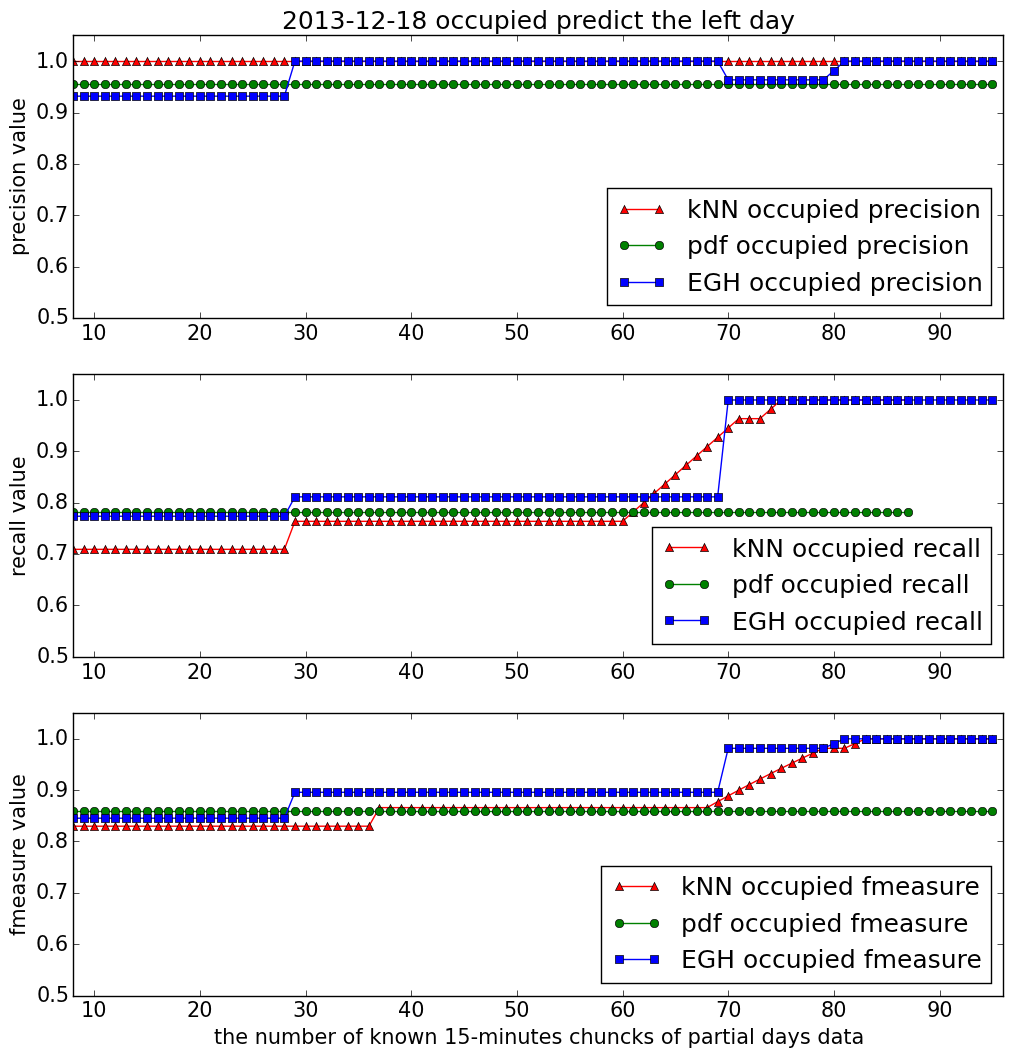
\includegraphics[width=0.5\textwidth]{adlfigs/study14person12013-12-18occupied.png} 
\caption{Study 14 Precision recall and f-measure comparison of three approaches.
person1 occupied 12/18/2014.}
\label{fig_study14}
\end{figure}
\fi


\subsection{Occupancy Prediction of Residential Buildings}
Based on individual prediction results, we deduce when a house is occupied
using logic OR operations on the prediction results of two persons. 
The whole house occupancy prediction results are listed in 
Table~\ref{tab_individualResults} and marked in bold. 
In Study10, the precision, recall, and fmeasure values of the whole house are 0.92, 0.92 and 0.91, respectively,  
which are higher than the values from the kNN approach of 0.91, 0.90 and 0.91, and of the SVR approach 0.79, 0.74 and 0.74. Similarly, the mixture EGH model outperforms kNN in Study11. 
Note that in Study 11 on 02/04/2015, 
EGH does not perform as well as kNN on individuals
but performs a little bit better than kNN, and much better than SVR in occupancy prediction of the whole house. 
The reason behind this is because the activities of the two people inside the home 
are not synchronized. The mixture EGH model can predict the 
occupancy for each person and grasp each person's activities more accurately. 
%When applying the logic OR operations on these two persons, 
%for whole-house occupancy prediction. 
\subsection{Limitations of Mixture EGH Model}
Although the temporal mixture EGH model performs well on the datasets Study10 and Study11, 
the same is not true for the dataset Study14. 
Table~\ref{tab_resultsLimitation} shows that, 
in Study14, 
the mixture EGH model works better for the individual and whole-house occupancy predictions on 12/18/2013 but not on 12/19/2013 or 12/20/2013. 
We check the activities of both individuals on these two days 
and find that both of them went out again 
after coming back and staying home for a while.
Since the episodes of going out after coming back home from work 
do not occur frequently, mixture EGH cannot detect this pattern. Thus the occupancy prediction probability of these events 
is completely missing. However kNN performs well because it leverages all the 
historical data; therefore, even if the abnormal event occurs once, 
this prediction approach incorporates it and obtains the average value. 
To relax the limitations of abnormal events, 
we propose a hybrid model for prediction;
when deploying this occupancy prediction in reality, 
for example for a prediction that is 30 minutes ahead, 
just 15 minutes before the prediction, if a person goes out again after coming back, 
the deployed system switches to the kNN approach rather than the mixture EGH model for prediction. In such cases, this hybrid model can always get the best prediction results. 

\begin{table*}[!t]
%\vspace{0.2cm}
\hfill
%\begin{minipage}[t]{1.0\linewidth}%

\caption{Precision Recall F-measure of Individual and Whole House Occupancy Prediction in Study 14.}
\label{tab_resultsLimitation}
%\tbl{Precision Recall F-measure of Individual and Whole House Occupancy Prediction in Study 14.\label{tab_resultsLimitation}}{
%\begin{center}
%\makebox[\textwidth]{
\centering
\small
\setlength\tabcolsep{2pt}
\begin{tabular} {|l|l|l|l|l|l|l|l|l|l|l|l|}
\hline
\multirow{2}{*}{Dataset}&\multirow{2}{*}{Date}&\multirow{2}{*}{Person} & \multicolumn{3}{|c|}{EGH}&\multicolumn{3}{|c|}{kNN} & \multicolumn{3}{|c|}{SVM} \\
\cline{4-12}
&&& precision & recall &fmeasure &precision & recall & fmeasure &precision & recall & fmeasure  \\
\hline
\multirow{3}{*}{study14}  & 12/18/2013 & person2&  \textbf{0.91} &  \textbf{0.91} &  \textbf{0.89} & 0.87 & 0.87 & 0.84 & 0.73 & 0.77 & 0.71\\
\cline{2-12}
& 12/18/2013 & person1&  \textbf{0.92} &  \textbf{0.92} &  \textbf{0.91} & 0.90 & 0.90 & 0.89 & 0.73 & 0.76 & 0.71 \\
\cline{2-12}
& 12/19/2014 & person2& 0.86 & 0.86 & 0.85  & \textbf{0.90} & \textbf{0.90} & \textbf{0.88} & 0.73 & 0.76 & 0.71\\
\cline{2-12}
& 12/19/2014 & person1& 0.85 & 0.84 & 0.84  & \textbf{0.86} & \textbf{0.86} & \textbf{0.85} & 0.73 & 0.76 & 0.71 \\
\cline{2-12}
& 12/20/2014 & person2& 0.92 & 0.94 & 0.92  & \textbf{0.98} & \textbf{0.97} & \textbf{0.97} & 0.75 & 0.79 & 0.75 \\
\cline{2-12}
& 12/20/2014 & person1& 0.90 & 0.91 & 0.90  & \textbf{0.95} & \textbf{0.95} & \textbf{0.95} & 0.75 & 0.79 & 0.75\\
\cline{2-12}
& 12/18/2013 & \textbf{wholehouse}&  \textbf{0.91}& \textbf{0.91} & \textbf{0.90} & 0.88	& 0.88 & 0.86 & 0.75 & 0.72 & 0.70 \\
\cline{2-12}
& 12/19/2013 & \textbf{wholehouse} & 0.841	& 0.845 & 0.838&  \textbf{0.848}& \textbf{0.853} & \textbf{0.842} & 0.79 & 0.74 & 0.74 \\
\cline{2-12}
& 12/20/2013 & \textbf{wholehouse} & 0.92	& 0.90 & 0.90&  \textbf{0.94}& \textbf{0.93} & \textbf{0.93} & 0.74 & 0.72 & 0.70 \\
\hline
\end{tabular}
%}
%\end{center}
%\end{minipage}%
%\hfill%
\end{table*}
\subsection{House Occupancy Prediction 30 Minutes Ahead with Hybrid Approach}
To preheat the house, we need to evaluate how much time in advance to automatically turn on/off HVAC, and the advance notice time estimation is given in~\cite{scott2011preheat}. 
Here we use prediction of 30 minutes ahead of time house occupancy. 
%because it is reasonable for preheating. 
We compare the receiver operating characteristic (ROC curve) of three approaches: mixture EGH model,  kNN, and a hybrid approach of the mixture EGH model and kNN. 
In this hybrid approach, 
we set mixture EGH results as the baseline, 
then replace the values of the mixture model by the values from kNN model 
in the following two situations: 
1) After a person comes back home; and 2) When the prediction probability of kNN is greater than 0.8. 
Figure~\ref{fig_rocresults_1}, ~\ref{fig_rocresults_2}, and~\ref{fig_rocresults_3} illustrate the ROC curve of the whole house occupancy prediction on 02/20/2014 of dataset Study10, 02/04/2014 of dataset Study 11 
and 12/20/2013 of dataset Study14, respectively.  
The red and green lines represents the kNN and mixture EGH models; 
the blue line denotes the hybrid approach. 
The ROC curves show that the hybrid approach always has the largest area, namely 
0.96, 0.92 and 0.92, 
which indicate that the hybrid approach always performs best. 
%\begin{figure}[h]
	\centering{
		\begin{tabular}{cccc}		
		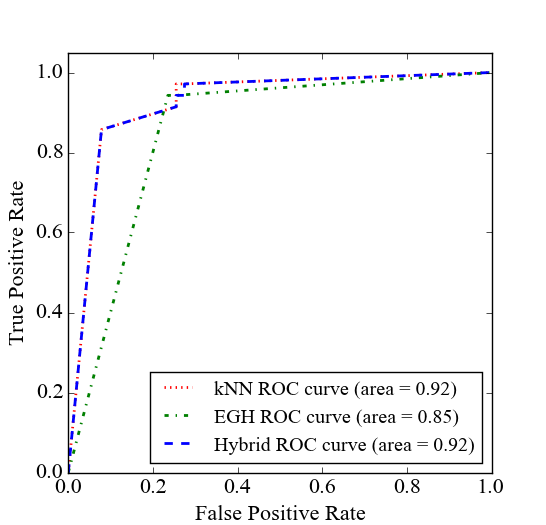
\includegraphics[width=0.5\textwidth]{adlfigs/study10ROC_02202014.png} &
		\tabular newline
		(a)\tabularnewline
		\end{tabular}
		}
	\caption{
	ROC curve of house occupancy prediction in Study10 (02/20/2014).}
	\label{fig_rocresults_1}
\end{figure}

\begin{figure}[h]
	\centering{
		\begin{tabular}{cccc}		
		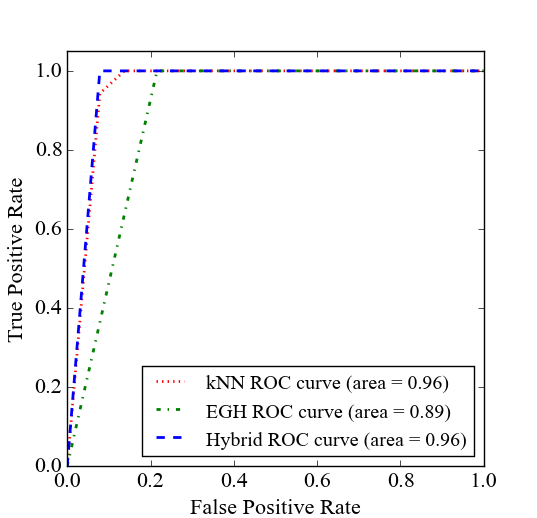
\includegraphics[width=0.5\textwidth]{adlfigs/study11ROC_02042014.png} &
		\tabularnewline
		((b)\tabularnewline
		\end{tabular}
		}
	\caption{
	ROC curve of house occupancy prediction in Study11 (02/04/2014).
}
	\label{fig_rocresults_2}
\end{figure}

\begin{figure}[h]
	\centering{
		\begin{tabular}{cccc}		
		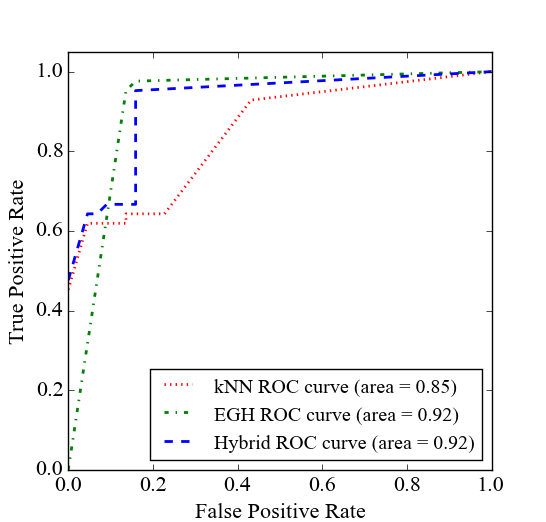
\includegraphics[width=0.5\textwidth]{adlfigs/study14ROC_12202013.png}
		\tabularnewline
		(c) \tabularnewline
		\end{tabular}
		}
	\caption{
	ROC curve of house occupancy prediction in (c) Study14 (12/20/2013).
}
	\label{fig_rocresults_3}
\end{figure}
\begin{figure}[h]
	\centering{
		\begin{tabular}{cccc}		
		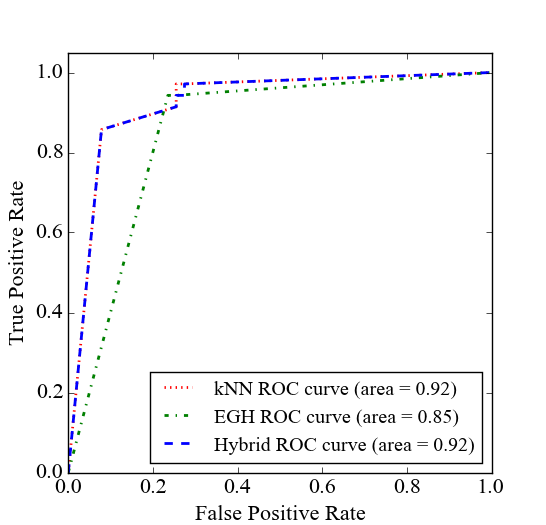
\includegraphics[width=0.5\textwidth]{adlfigs/study10ROC_02202014.png} &
		\tabularnewline
		(a)\tabularnewline
		\end{tabular}
		}
	\caption{
	ROC curve of house occupancy prediction in Study10 (02/20/2014).}
	\label{fig_rocresults_1}
\end{figure}

\begin{figure}[h]
	\centering{
		\begin{tabular}{cccc}		
		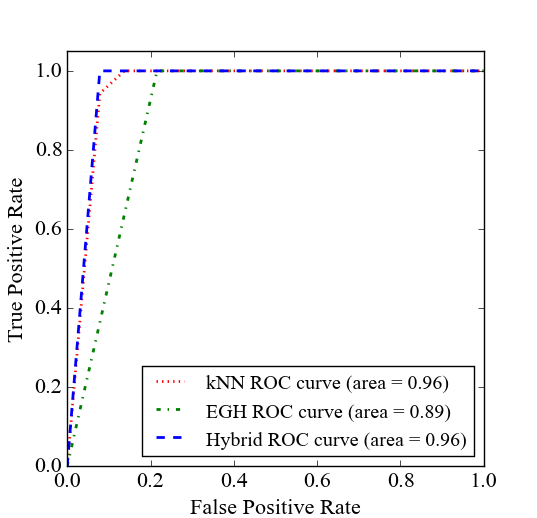
\includegraphics[width=0.5\textwidth]{adlfigs/study11ROC_02042014.png} &
		\tabularnewline
		((b)\tabularnewline
		\end{tabular}
		}
	\caption{
	ROC curve of house occupancy prediction in Study11 (02/04/2014).
}
	\label{fig_rocresults_2}
\end{figure}

\begin{figure}[h]
	\centering{
		\begin{tabular}{cccc}		
		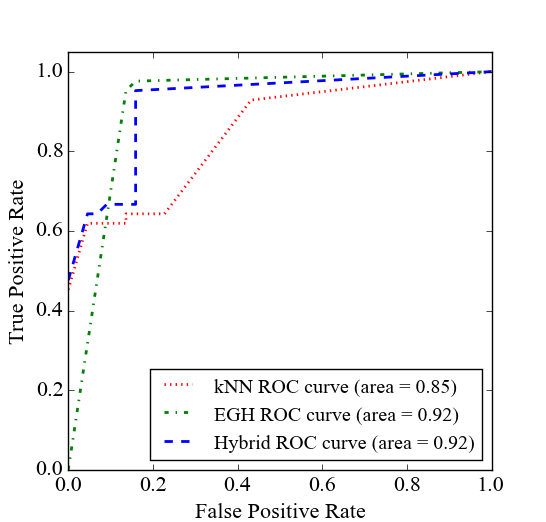
\includegraphics[width=0.5\textwidth]{adlfigs/study14ROC_12202013.png}
		\tabularnewline
		(c) \tabularnewline
		\end{tabular}
		}
	\caption{
	ROC curve of house occupancy prediction in (c) Study14 (12/20/2013).
}
	\label{fig_rocresults_3}
\end{figure}



%Also, we compare the 30 minutes whole house precision/recall/f-measure with the ROC curve, 
%the kNN ROC has a larger area even if EGH approach performs better on study10 and study11. 

%It depicts that ROC curve of mixture EGH model occupied larger area 0.92 than that from kNN approach 0.85. 
%We observe that although the precision/recall/fmeasure values are very close as in table~\ref{tab_individualResults}. 
%This hints that although the precision/recall/fmeasure results are competitive, 
%mixture EGH model can separate the occupancy and un-occupancy more sharply. 



%There are three test days in the dataset study14, 
%EGH outperforms kNN on the first day. 
%It's a tie on the second day. 
%The only exception on these datasets is the last day's experiment on study14, 
%kNN performs better because EGH mixture model currently
%only works on one-time even prediction. 


